% Chapter Template

\chapter{Methods and Materials} % Main chapter title

\label{Chapter 3} % Change X to a consecutive number; for referencing this chapter elsewhere, use \ref{ChapterX}

This chapter describes how work on the project was conducted. It does this by first describing the methodology used, then by following with the hardware and software used.

%----------------------------------------------------------------------------------------
%	SECTION 1
%----------------------------------------------------------------------------------------

\section{Methodology}

\label{Ch3 Sec1}

This project included several states, in which, debugging skills and a deep programming knowledge base was necessary. While debugging there were a few techniques used that enabled fast and more accurate pinpointing of the offending pieces of hardware. Chief among these debugging techniques was to visually expose relevant signals. By exposing a signal in real time it could be quickly and easily verified as either working or not working. Should this fail, another useful debugging technique was to simulate the modules with report statements. While this was not always viable, it did allow for much more real time data to be exposed; it also allowed exact inputs to the hardware to be monitored. The final debugging technique used was to reduce the complexity of the hardware. By removing more complex elements of the hardware it is possible to isolate the issue and then fix it.

\section{Materials}

\label{Ch3 Sec2}

%-----------------------------------
%	SUBSECTION 1
%-----------------------------------
\subsection{Hardware Used}

\label{Ch3 Sec2 Sub1}

During the development of the project several pieces of hardware was used, this hardware was used to create interact and program the MEGA65. In addition to this some of the work on the project required specific hardware to function in order for full functionality of the MEGA65 to be present. This hardware is listed as follows:\\

\begin{itemize}
\item{Digilent Nexys 4 DDR Artix-7 FPGA Trainer Board: This FPGA development board, as seen in figure \ref{fig:nexys4ddr}, was one of the vital components while conducting this project. It was used as the remappable hardware, on which, the MEGA65 prototypes could be tested.}
\item{Acer Aspire V Nitro: This laptop, as seen in figure \ref{fig:aspirevnitro}, was the most important piece of hardware used in this project. This piece of hardware was used to interface between the FPGA as well as make changes to the MEGA65 hardware.}
\item{Dell UltraSharp 2408WFP 24-inch LCD Monitor: This monitor, while not critical, was a required piece of hardware. This was used to host the VGA output from the MEGA65.}
\item{Dell KB1421 Keyboard: Much like the monitor, this piece of hardware was not critical but without it, or a similar product, progress on the project would be exceedingly difficult.}
\item{SanDisk Ultra 16Gb MicroSDHC Micro SD card: This SD card, like the keyboard and monitor, was not critical, it was necessary for full operation of the MEGA65 however.}
\end{itemize}

\begin{figure}
  \centering
  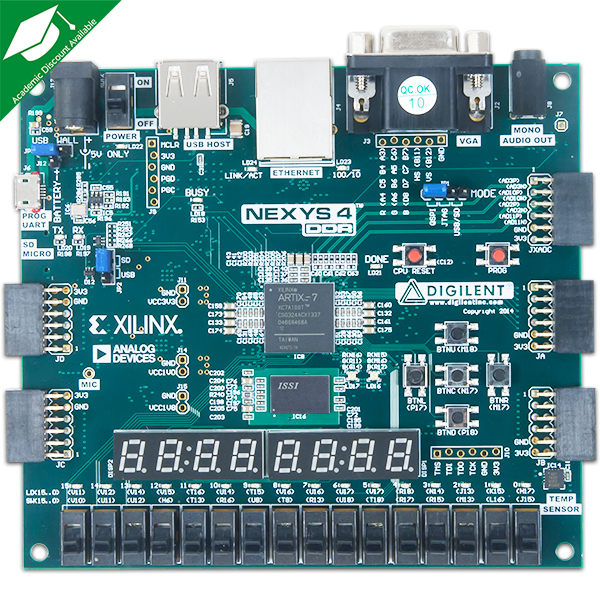
\includegraphics[width=0.75\linewidth]{nexys4ddr}
  \caption{The Nexys 4 DDR Artix-7 FPGA Trainer Board}
  \label{fig:nexys4ddr}
\end{figure}

\begin{figure}
  \centering
  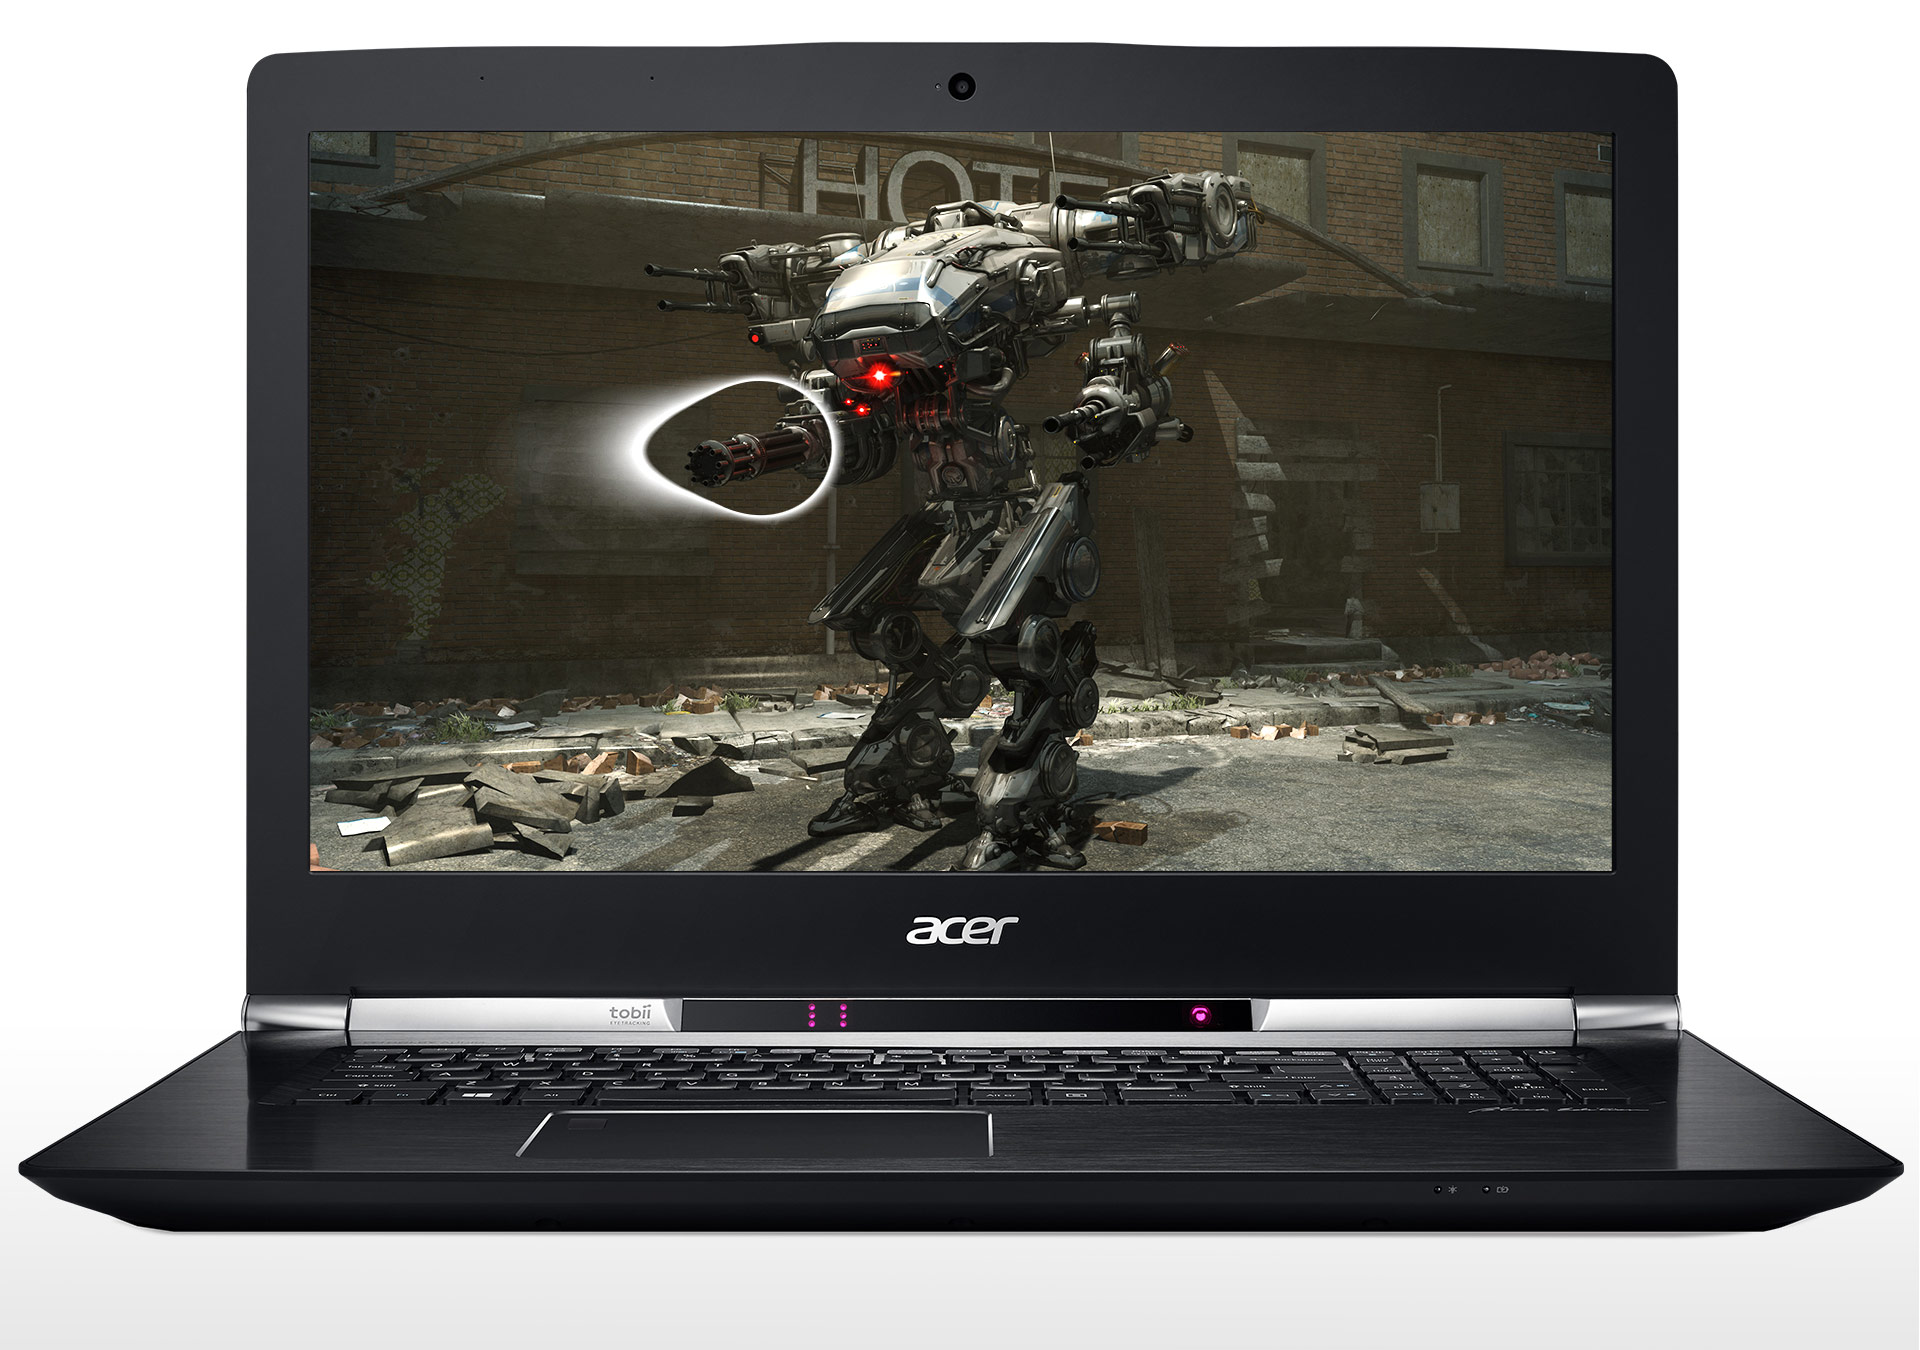
\includegraphics[width=0.75\linewidth]{aspirevnitro}
  \caption{The Acer Aspire V Nitro Laptop}
  \label{fig:aspirevnitro}
\end{figure}

%-----------------------------------
%	SUBSECTION 1
%-----------------------------------
\subsection{Software Used}

\label{Ch3 Sec2 Sub2}

During development of the MEGA65 several software packages were used in order to interact with the hardware listed above. These packages include:\\

\begin{itemize}
\item{Ubuntu 18.04: This operating system was required for work on the project. It was through it that commands required to program and interact with the FPGA were able to function.}
\item{Vivado HLx Webpack Edition: The development tools that this webpack provided was critical for the function of the MEGA65. These tools were used to program and make changes to the FPGA.}
\item{Git: This version control tool, while not necessary, was extremely useful. This allowed changes to be tracked and shared between developers on the project. The hosted repositories are found on the GitHub website}
\item{GHDL: This VHDL simulation software was very useful when debugging during the project. It allowed for more easily accessible variables during run time.}
\end{itemize}
